\section{Resultados}
\label{sec:resultados}

\subsection{Baselines Cl\'asicos}
Los tres modelos cl\'asicos evaluados sobre el dataset Iris completo (105 train / 45 test) alcanzaron un rendimiento pr\'acticamente id\'entico: SVM-RBF, MLP y KNN obtuvieron un \textit{accuracy} de 93.33\% y F1-score macro de $\sim$0.933. Esta frontera cl\'asica establece el techo de referencia contra el cual se contrastan los modelos cu\'anticos.

\subsection{Modelo Variacional Corregido (VQC)}
El VQC ajustado (300 iteraciones m\'aximas de COBYLA, 3 semillas iniciales distintas) fue evaluado sobre el dataset Iris completo. Los resultados individuales por semilla fueron:

\begin{table}[H]
\centering
\caption{Resultados del VQC corregido por semilla de inicializaci\'on.}
\label{tab:vqc_seeds}
\small
\begin{tabular}{@{}cccc@{}}
\toprule
\textbf{Semilla} & \textbf{Accuracy} & \textbf{Iteraciones} & \textbf{Tiempo (s)} \\
\midrule
42  & 55.56\% & 152 & 36.1 \\
123 & 60.00\% & 164 & 41.1 \\
789 & 46.67\% & 130 & 32.5 \\
\midrule
\textbf{Mejor} & \textbf{60.00\%} & 164 & 41.1 \\
\bottomrule
\end{tabular}
\end{table}

\noindent El mejor modelo alcanz\'o un F1-score macro de 0.5051. Como muestra la Figura~\ref{fig:baseline}, el VQC mejorado a\'un se sit\'ua muy por debajo de la frontera cl\'asica (SVM 93.33\%), evidenciando que el \textit{loss landscape} variacional presenta m\'inimos locales dif\'iciles de superar incluso con iteraciones ampliadas.

\begin{figure}[H]
    \centering
    
\includegraphics[width=\linewidth]{graficos/exp1_baseline_corregido.png}
    \caption{M\'etricas de exactitud del VQC mejorado y la frontera l\'imite cl\'asica (SVM 93.33\%).}
    \label{fig:baseline}
\end{figure}

\subsection{Verificaci\'on Geom\'etrica del Ruido (Estado de Bell)}
La preparaci\'on del estado m\'aximamente entrelazado $|\Phi^+\rangle$ sobre \texttt{ibm\_fez} arroj\'o una \textbf{fidelidad de 0.9834}, valor que confirma la alta calidad del hardware Heron r2 para operaciones de entrelazamiento b\'asico. La Figura~\ref{fig:bell_circuit} muestra el circuito de Bell utilizado, descompuesto en sus puertas b\'asicas (H + CNOT). Los histogramas de probabilidad (Figura~\ref{fig:bell}) muestran una distorsi\'on menor respecto a la distribuci\'on ideal del simulador, con peque\~nas fugas hacia los estados $|01\rangle$ y $|10\rangle$ atribuibles a errores SPAM y decoherencia $T_1$.

\begin{figure}[H]
    \centering
    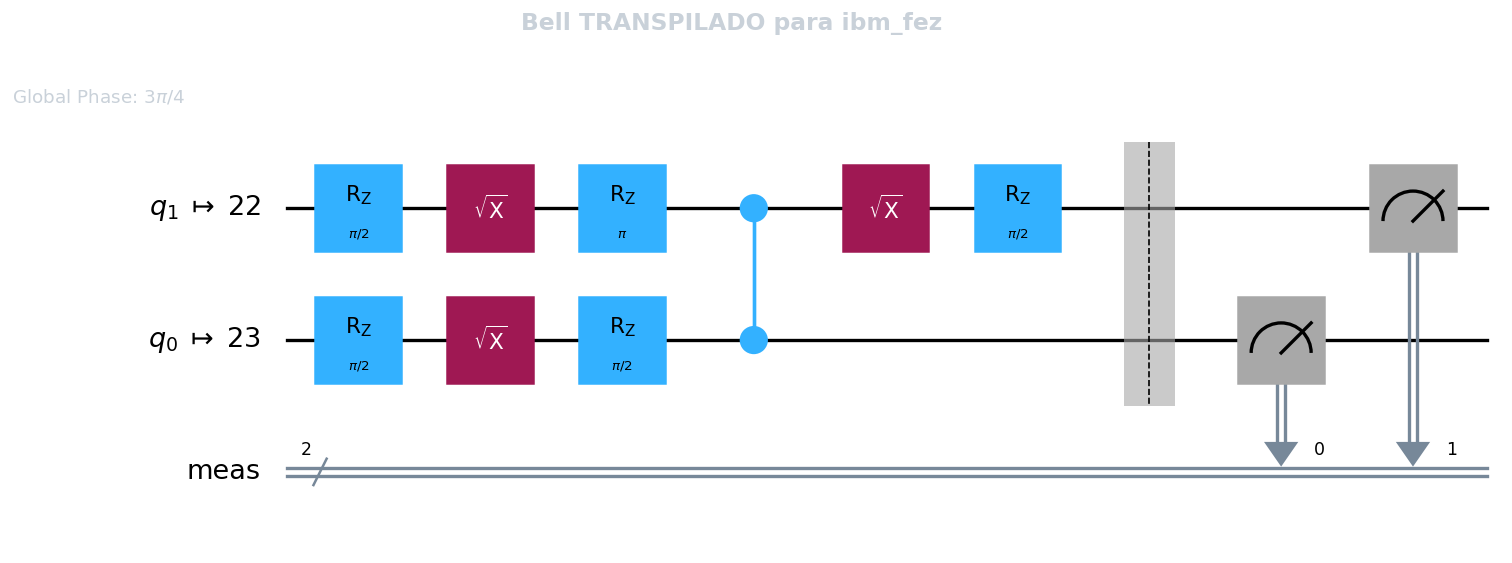
\includegraphics[width=0.85\linewidth]{graficos/vis_bell_circuit_2.png}
    \caption{Circuito de Bell descompuesto: compuerta Hadamard sobre $q_0$ seguida de CNOT($q_0$, $q_1$), que genera el estado $|\Phi^+\rangle = \frac{1}{\sqrt{2}}(|00\rangle + |11\rangle)$.}
    \label{fig:bell_circuit}
\end{figure}

\begin{figure}[H]
    \centering
    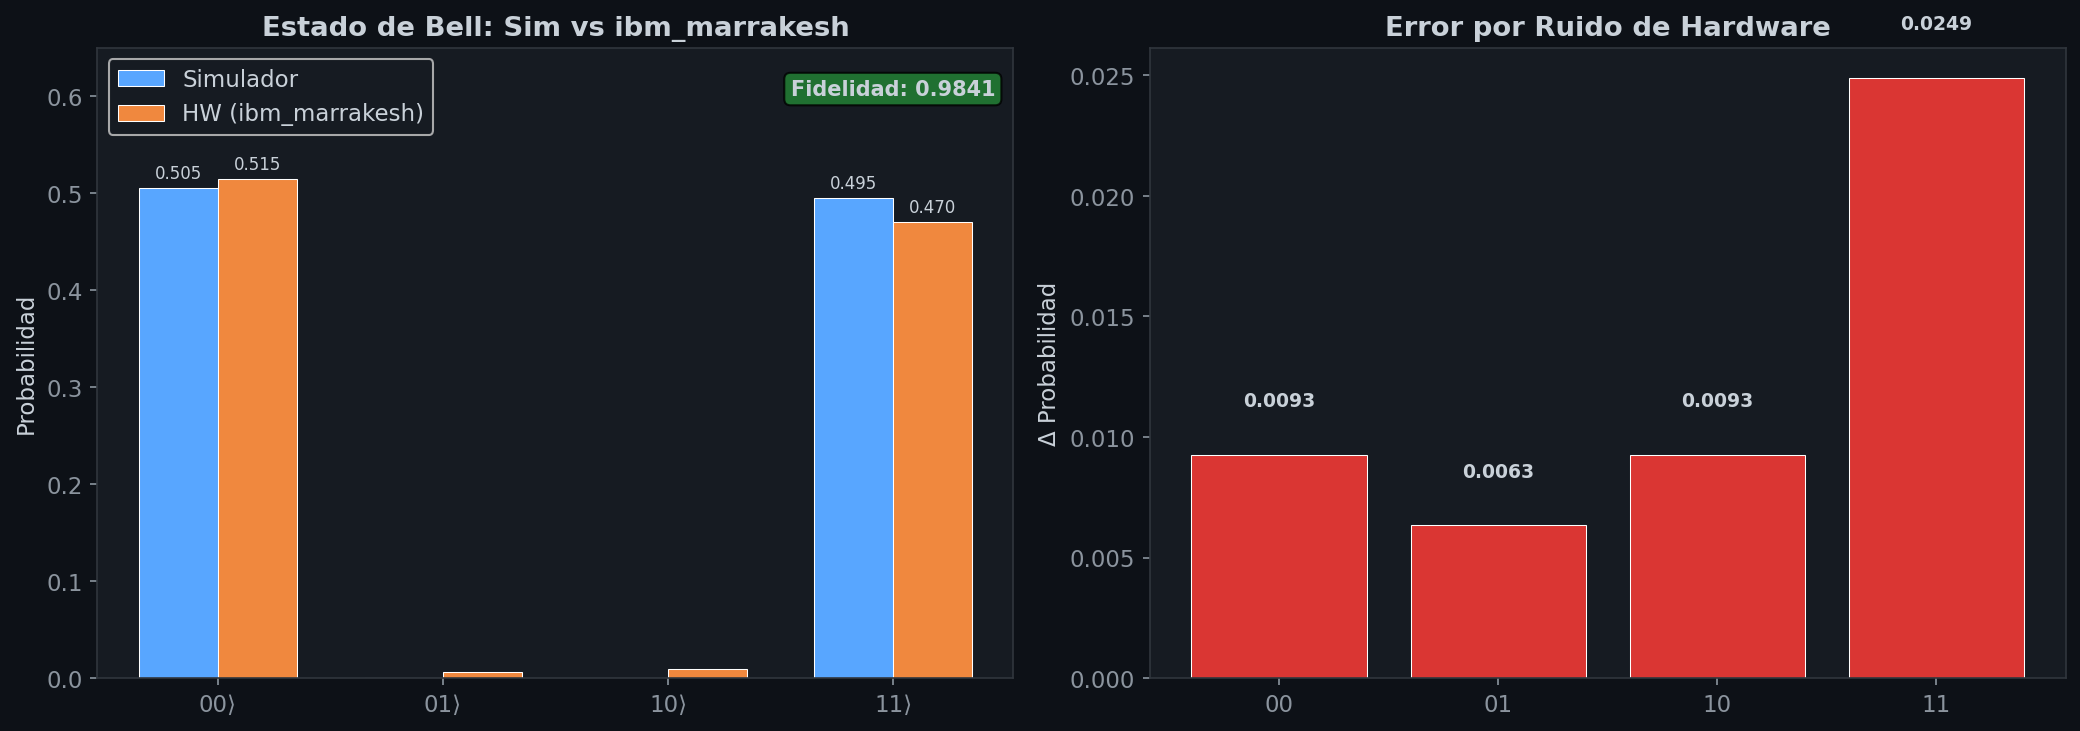
\includegraphics[width=\linewidth]{graficos/exp2_bell_state.png}
    \caption{Comparaci\'on de distribuciones de probabilidad entre \textit{Statevector} e \textit{ibm\_fez} para el estado de Bell. Fidelidad: 0.9834.}
    \label{fig:bell}
\end{figure}

\subsection{Kernel QSVC: Simulador vs. Hardware}
Este experimento constituye el n\'ucleo de la investigaci\'on. El kernel cu\'antico se construye mediante el circuito \textit{compute-uncompute} (Figura~\ref{fig:kernel_circuit}), donde se aplica el feature map $U_\phi(\mathbf{x}_i)$ seguido del inverso $U_\phi^\dagger(\mathbf{x}_j)$, y la probabilidad de medir el estado $|0000\rangle$ determina la similitud $K(\mathbf{x}_i, \mathbf{x}_j)$.

\begin{figure}[H]
    \centering
    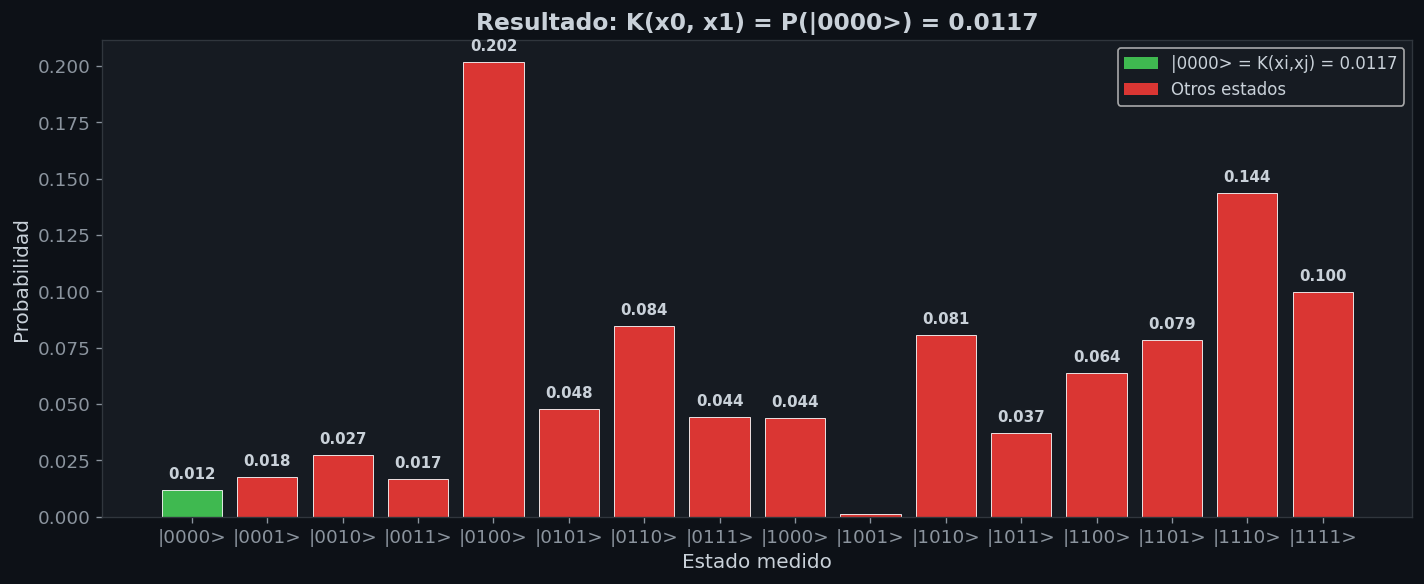
\includegraphics[width=\linewidth]{graficos/vis6_compute_uncompute_2.png}
    \caption{Circuito \textit{compute-uncompute} para el c\'alculo del kernel cu\'antico: $K(\mathbf{x}_i, \mathbf{x}_j) = |\langle 0^n | U_\phi^\dagger(\mathbf{x}_j) \cdot U_\phi(\mathbf{x}_i) | 0^n \rangle|^2$. Se muestra con datos reales del dataset Iris.}
    \label{fig:kernel_circuit}
\end{figure}

\noindent La QSVC fue evaluada primero con el dataset completo en simulador (Acc = 77.78\%, F1 = 0.777), y luego con el subset reducido (13 train / 9 test) tanto en simulador como en hardware real. Los resultados revelan una \textbf{degradaci\'on significativa} del hardware frente al simulador:

\begin{table}[H]
\centering
\caption{QSVC sobre subset reducido: simulador vs. hardware.}
\label{tab:qsvc_hw}
\small
\begin{tabular}{@{}lccc@{}}
\toprule
\textbf{Entorno} & \textbf{Accuracy} & \textbf{F1 (macro)} & \textbf{Tiempo} \\
\midrule
Simulador (subset) & 33.33\% & 0.324 & 0.46s \\
Hardware (ibm\_fez) & 11.11\% & 0.111 & 182s \\
\bottomrule
\end{tabular}
\end{table}

\noindent Como evidencia la Figura~\ref{fig:qsvc_kernel}, el simulador ya muestra un rendimiento deficiente (33.33\%) debido a la insuficiencia muestral, pero el hardware degrada el resultado hasta un 11.11\%, equivalente a clasificar correctamente apenas 1 de 9 muestras de prueba. Esta ca\'ida de $\sim$22 puntos porcentuales demuestra que el ruido NISQ \textbf{s\'i} constituye un factor de degradaci\'on significativo, a\'un cuando opera sobre un kernel ya debilitado por la escasez de datos.

\begin{figure}[H]
    \centering
    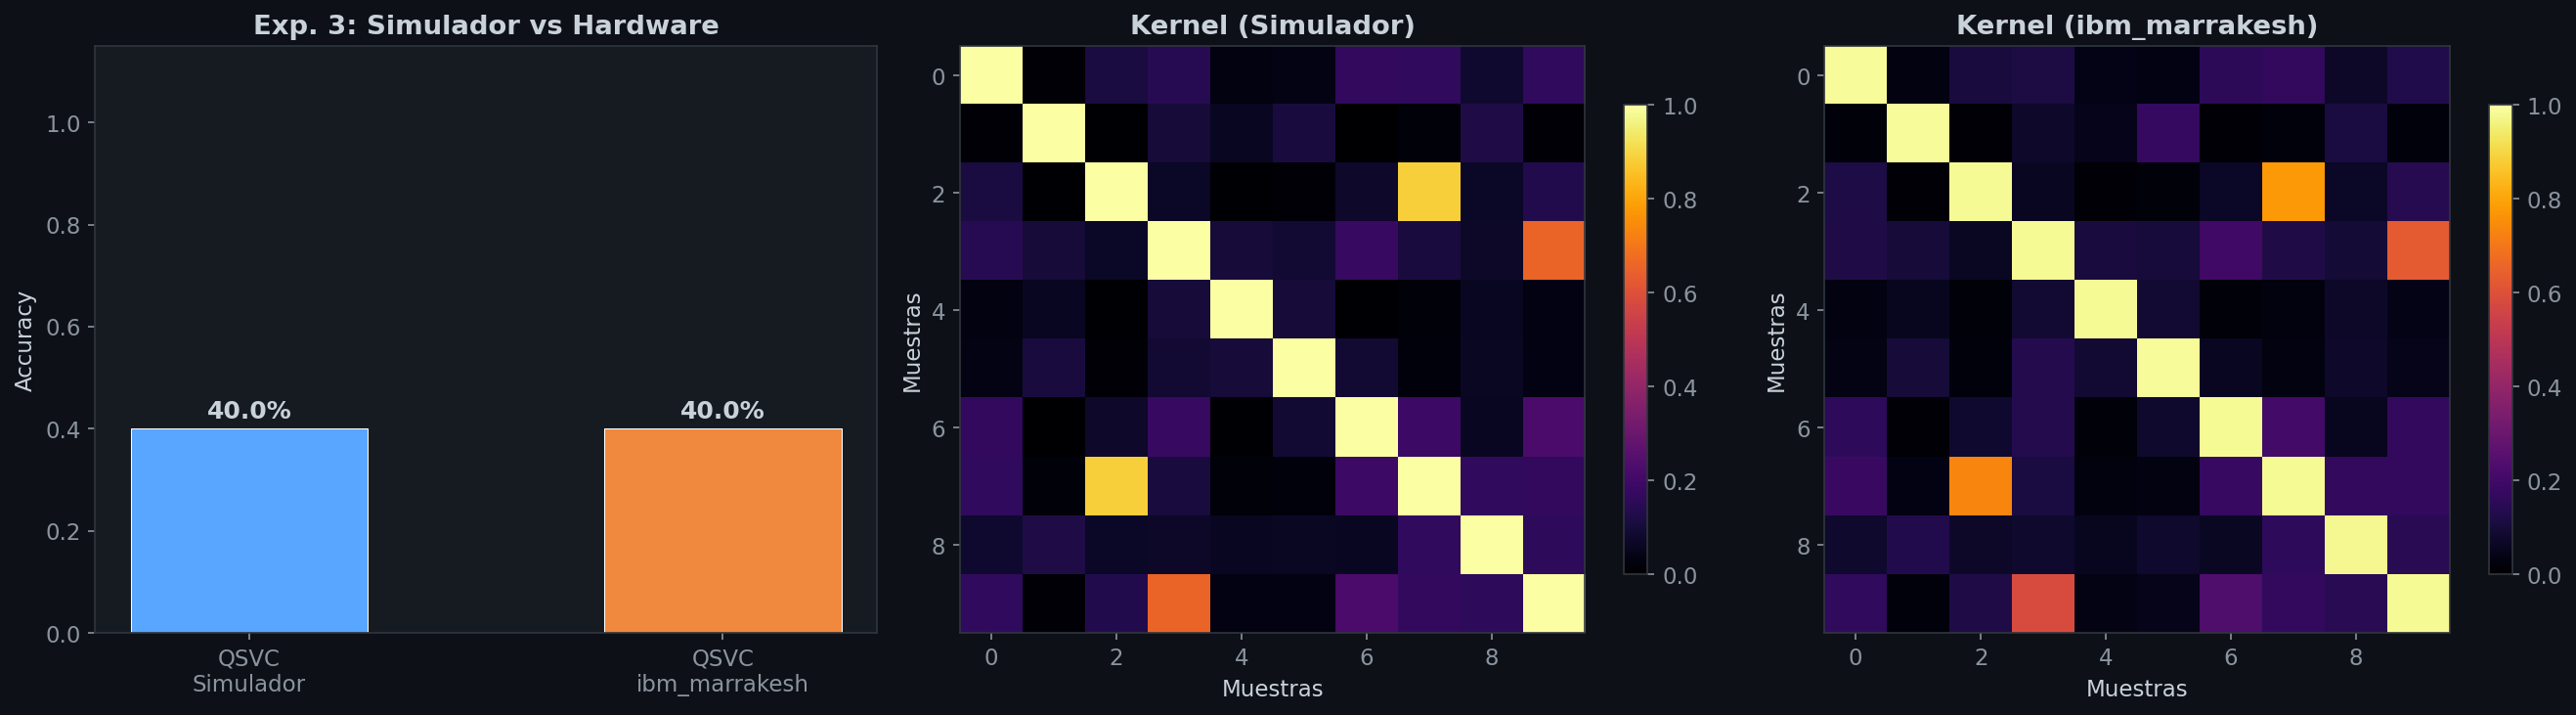
\includegraphics[width=\linewidth]{graficos/exp3_qsvc_hw_vs_sim.png}
    \caption{Matrices de similitud del kernel cu\'antico y rendimiento comparado entre simulador (33.33\%) y hardware real (11.11\%) bajo restricci\'on estricta de muestra.}
    \label{fig:qsvc_kernel}
\end{figure}

\subsection{Mitigaci\'on TREX}
La implementaci\'on de la t\'ecnica de mitigaci\'on local TREX (Figura~\ref{fig:trex}) no logr\'o mejorar el resultado en hardware, manteni\'endose en un \textbf{11.11\%} de accuracy, id\'entico al escenario sin mitigaci\'on. Esto indica que, bajo condiciones de degradaci\'on tan severa (combinaci\'on de escasez muestral y ruido), las correcciones algor\'itmicas de lectura resultan insuficientes para recuperar informaci\'on \'util de un kernel geom\'etricamente colapsado.

\begin{figure}[H]
    \centering
    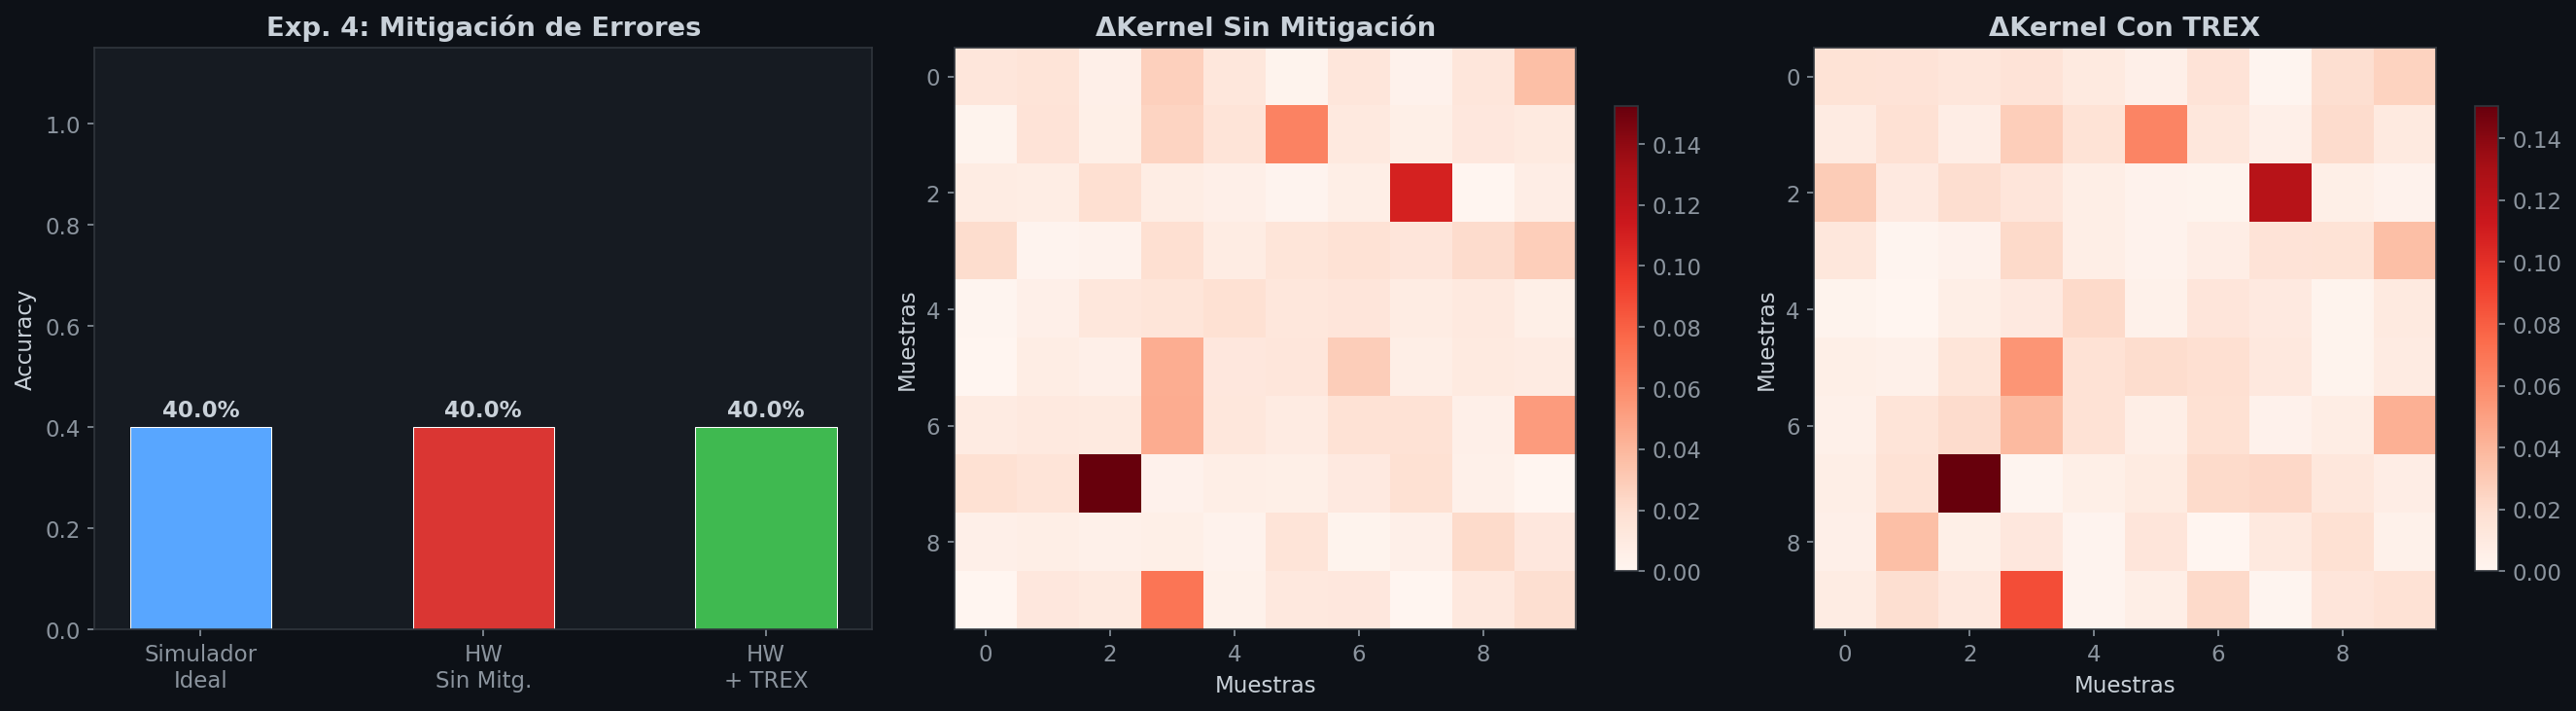
\includegraphics[width=\linewidth]{graficos/exp4_error_mitigation.png}
    \caption{Estabilidad de predicci\'on post-procesamiento TREX. Accuracy invariable (11.11\%) respecto al escenario sin mitigaci\'on.}
    \label{fig:trex}
\end{figure}

\subsection{Clasificaci\'on MNIST en Hardware}
El dataset binario MNIST (0 vs. 1), comprimido a 4 dimensiones via PCA (73.44\% de varianza capturada), present\'o un comportamiento particularmente interesante (Figura~\ref{fig:mnist}):

\begin{table}[H]
\centering
\caption{Resultados MNIST: cl\'asico, simulador y hardware.}
\label{tab:mnist}
\small
\begin{tabular}{@{}lccc@{}}
\toprule
\textbf{Modelo} & \textbf{Accuracy} & \textbf{F1} & \textbf{Tiempo} \\
\midrule
SVM-RBF cl\'asico       & 100.00\% & 1.000 & 0.01s \\
QSVC simulador          & 77.78\%  & 0.775 & 0.43s \\
QSVC hardware (ibm\_fez) & 88.89\% & 0.889 & 205s \\
\bottomrule
\end{tabular}
\end{table}

\noindent De manera at\'ipica, el hardware real super\'o al simulador (88.89\% vs. 77.78\%). Este fen\'omeno puede atribuirse a la naturaleza estoc\'astica del muestreo cu\'antico en problemas de clasificaci\'on binaria con pocas muestras, donde las perturbaciones del ruido pueden, por azar estad\'istico, favorecer la separabilidad de las clases.

\begin{figure}[H]
    \centering
    
\includegraphics[width=\linewidth]{graficos/exp5_mnist_hardware.png}
    \caption{Desempe\~no comparativo de clasificaci\'on binaria MNIST (0 vs. 1) super-reducido (PCA a 4D).}
    \label{fig:mnist}
\end{figure}

\subsection{Resumen Comparativo General}

La Tabla~\ref{tab:resumen} consolida todos los resultados experimentales, y la Figura~\ref{fig:radar} presenta la visi\'on panor\'amica mediante un espectro radial.

\begin{table}[H]
\centering
\caption{Resumen comparativo de todos los modelos evaluados.}
\label{tab:resumen}
\footnotesize
\begin{tabular}{@{}llccl@{}}
\toprule
\textbf{Tipo} & \textbf{Modelo} & \textbf{Acc.} & \textbf{F1} & \textbf{Entorno} \\
\midrule
Cl\'as.  & SVM-RBF (Iris)      & 93.3\% & .933 & Local \\
Cl\'as.  & MLP (Iris)          & 93.3\% & .933 & Local \\
Cl\'as.  & KNN (Iris)          & 93.3\% & .933 & Local \\
\midrule
Sim.    & VQC (Iris)          & 60.0\% & .505 & Statevector \\
Sim.    & QSVC (Iris full)    & 77.8\% & .777 & Statevector \\
Sim.    & QSVC (Iris sub.)    & 33.3\% & .324 & Statevector \\
\midrule
HW      & QSVC sin mitg.      & 11.1\% & .111 & ibm\_fez \\
HW      & QSVC + TREX         & 11.1\% & .111 & ibm\_fez \\
\midrule
Cl\'as.  & SVM-RBF (MNIST)     & 100\%  & 1.00 & Local \\
Sim.    & QSVC (MNIST)        & 77.8\% & .775 & Statevector \\
HW      & QSVC (MNIST)        & 88.9\% & .889 & ibm\_fez \\
\bottomrule
\end{tabular}
\end{table}

\begin{figure}[H]
    \centering
    
\includegraphics[width=\linewidth]{graficos/resumen_final_radar.png}
    \caption{Radar de rendimiento: Accuracy y F1 (macro) para todos los escenarios evaluados.}
    \label{fig:radar}
\end{figure}
